\chapter{Testing}

\section{Original Data}

Here we will explore the results of different classifiers and active learning strategies on the original data. The original data consisted of data shown previously in Figure \ref{fig:original_english_counts} and discretely in Table \ref{tab:en_data_counts} in Appendix \ref{app:attachments}. 

\subsection{Active Learning with PWC and RBF Kernel}

In Figure \ref{fig:plot_all_results_rbf} we have the train and test errors for four different active learning sampling strategies. XPAL appears to perform slightly better than PAL but not significantly better. With our data we found that PAL runs slower than xPAL, which was unexpected based on the mean computation time results published by \cite{kottke2021toward}. We expect this drop in calculation time is a result of the high dimensional data.

We weren't satisfied with the testing error which leveled out to about 70\% for each sampling strategy. PAL and xPAL were able to rapidly reduce the testing error early on in the training process while random selection and QBC weren't able to determine the data with the highest information gain. 

\begin{figure}[ht]
  \centering
  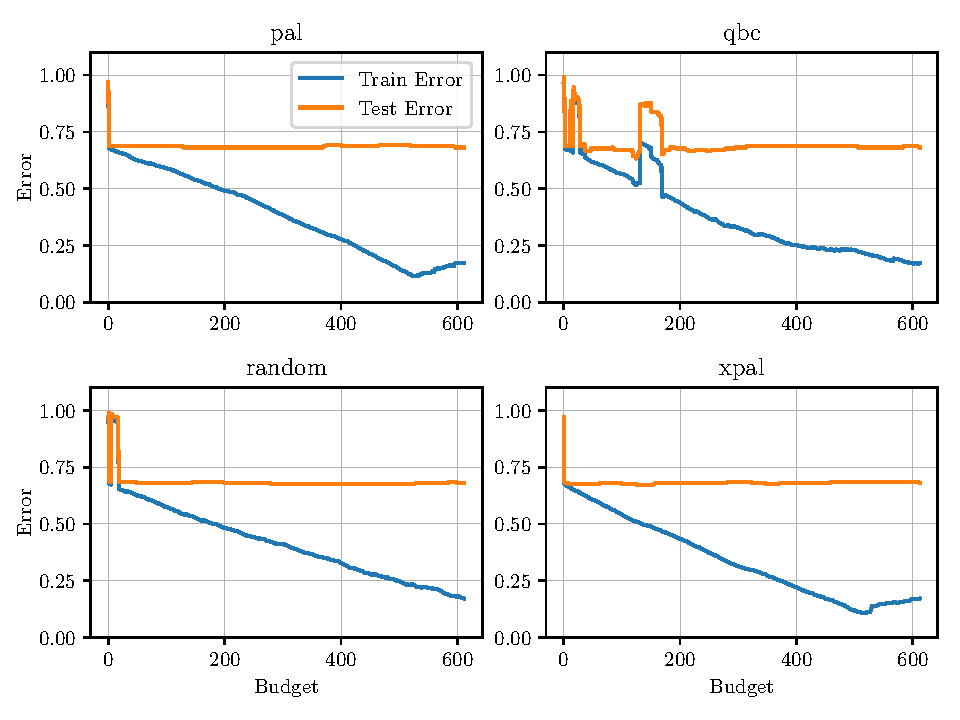
\includegraphics[width=\scale\textwidth]{../img/plot_all_results_rbf.pdf}
  \caption{Train and test error using different query strategies and RBF kernel for the PWC classifier.}
  \label{fig:plot_all_results_rbf}
\end{figure}

The radial bias function (RBF) kernel is a popular kernel function. It is defined as:

\begin{equation}
    K(x_i, x_j) = \exp\left(- \frac{\left\| x_i - x_j \right\|^2}{2 \sigma^2}\right)
\label{eq:rbf_kernel}
\end{equation}

where $\sigma$ is a parameter that controls the smoothness of the kernel and $x_i$ and $x_j$ are the two points in the feature space to compare. As seen in the Figure \ref{fig:plot_all_results_rbf} when the PWC classifier uses the RBF kernel it doesn't perform well with this data.

\subsection{Active Learning with PWC and Cosine Kernel}

In Figure \ref{fig:plot_all_results_cosine} we have the train and test errors for the same four different active learning sampling strategies tested on the same data. The only change was that we used Cosine kernel instead of the RBF kernel.The Cosine kernel is another important kernel function that is used in many machine learning algorithms. It is defined as:

\begin{equation}
    K(x_i, x_j) = \frac{x_i \cdot x_j}{\left\| x_i \right\| \left\| x_j \right\|}
\label{eq:cosine_kernel}
\end{equation}

where $x_i$ and $x_j$ are the two points in the feature space to compare. We found that using the Cosine kernel reduced the test error across the board by $\sim$15\%.  

\begin{figure}[ht]
  \centering
  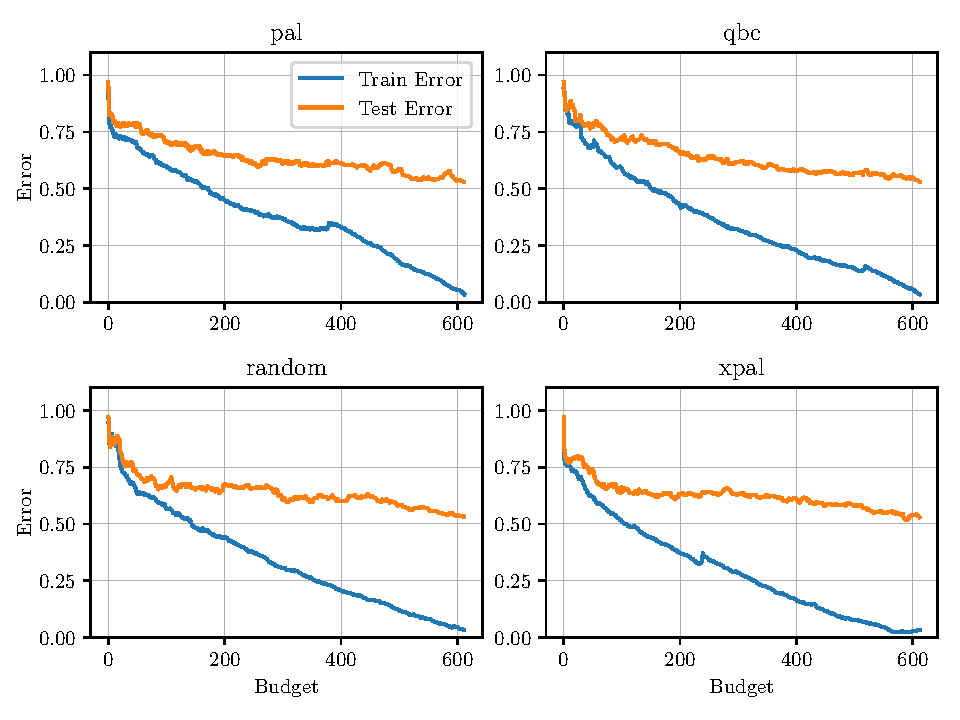
\includegraphics[width=\scale\textwidth]{../img/plot_all_results_cosine.pdf}
  \caption{Train and test error using different query strategies and Cosine kernel for the PWC classifier.}
  \label{fig:plot_all_results_cosine}
\end{figure}


In Figure \ref{fig:plot_all_results_cosine} PAL and xPAL were able to reduce the training error, by about 20\% and 25\% respectively, early in the training process compared to random selection and QBC. We also tested the other sampling strategies with the Cosine kernel and found that the results were similar. The other sampling strategies and their test data results are shown in Table \ref{fig:cos_test_results} along with the test data from Figure \ref{fig:plot_all_results_cosine}. 


\begin{figure}[ht]
    \centering
    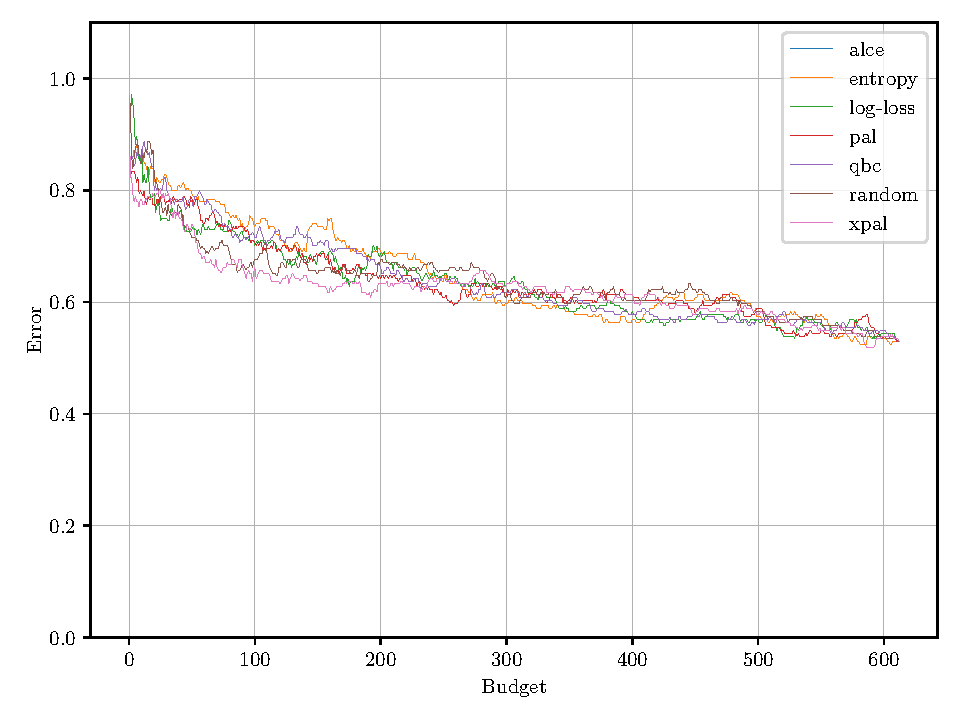
\includegraphics[width=\scale\textwidth]{../img/plot_kernel_cos_test_results.pdf}
    \caption{Comparing test error with one data split using different query strategies and Cosine kernel for the PWC classifier.}
    \label{fig:cos_test_results}
\end{figure}

We can see that the sampling strategies test performance converges over time (as we are using the same data and classifier) but xPAL appears to have an absolute minimum near the 600 budget mark in comparison to all sampling strategies. XPAL also appears to be performing well early on in the training process, in the 100-200 budget range. However, this test is only showing the results of one data split. We can get a better idea if we run more tests with different train-test splits and see how the results average out.

Figure \ref{fig:cos_test_results} shows that xPAL seems to be performing the best with our data but we wanted to see if we ran more tests with different train-test splits how the results would average out and which sampling strategy would perform the best on average. We ran 10 different data splits with each of the 7 sampling strategies and then took the average to get a smoother curve compared to the single run results shown in Figure \ref*{fig:cos_test_results}. The results for this experiment are shown in Figure \ref{fig:cos_avg_test_results}. 

It is clear in Figure \ref{fig:cos_avg_test_results} that xPAL is performing the best early on (budget from 0-100) in the sample selection process. XPAL selects the data that minimizes the test error and builds the strongest classifier quickly while it takes the other sampling strategies more data points to get to the same level of performance. Around the 100 budget mark we can see that the other selection strategies catch up to xPAL performance wise.

\begin{figure}[ht]
    \centering
    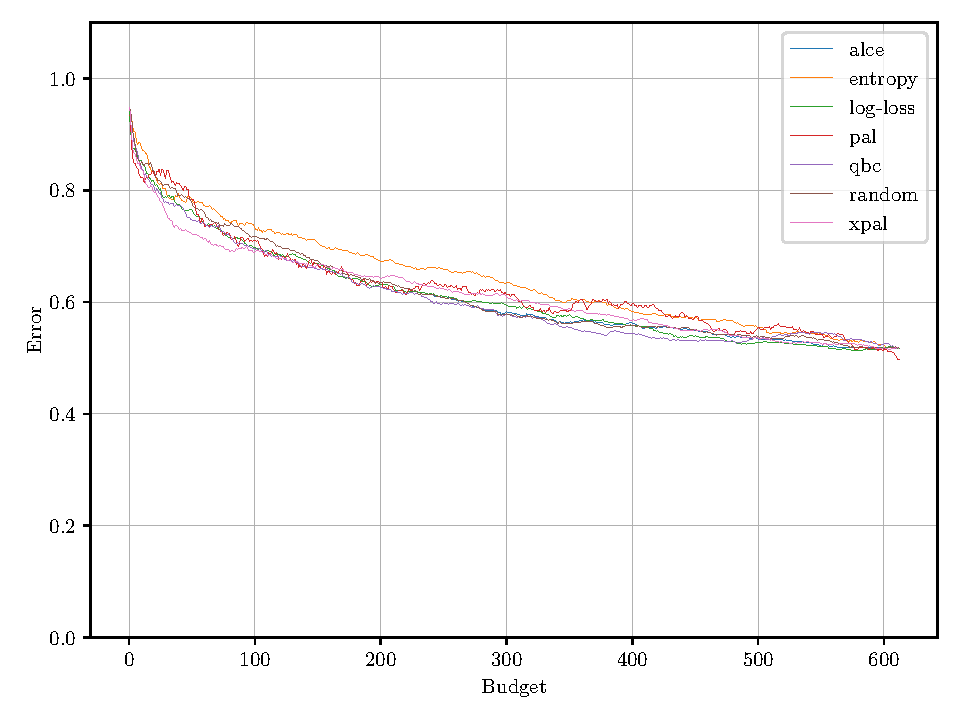
\includegraphics[width=\scale\textwidth]{../img/plot_kernel_cos_averaged_test_results.pdf}
    \caption{Comparing test error using different query strategies and Cosine kernel for the PWC classifier with results averaged over ten different data splits.}
    \label{fig:cos_avg_test_results}
\end{figure}


\subsection{Classifier Evaluation}

We also decided to test out some classifiers from the Scikit-Learn library to compare performances. Again we used the original data with the same TF-IDF vectorizer as used with the previous active learning models to stay consistent. It should be noted that cross validation was used here but it was not used in the previous sections.

The goal of this exploratory phase was to try and decide which classifier to conduct more thorough testing with. As a result, we didn't use GridSearchCV for each classifier at this stage and we mostly used the default parameters and their cross validation scores with all of the original data (i.e. additional data not included). In some cases where using weights was an option for the classifier we included the precomputed Cosine decay weights. A table of the parameters used for each classifier is shown in Appendix Table \ref{tab:explore_classifiers_params}.

The results for the different classifiers are shown in Figure \ref{fig:explore_classifiers}. In the box-plot, the whiskers extend from the box to the furthest data points that are within 1.5 times the inter-quartile range (IQR) of the box. Any data points that are beyond the whiskers are considered outliers and are plotted as individual points or symbols (diamonds) as seen in the figure.


\begin{figure}[ht]
  \centering
  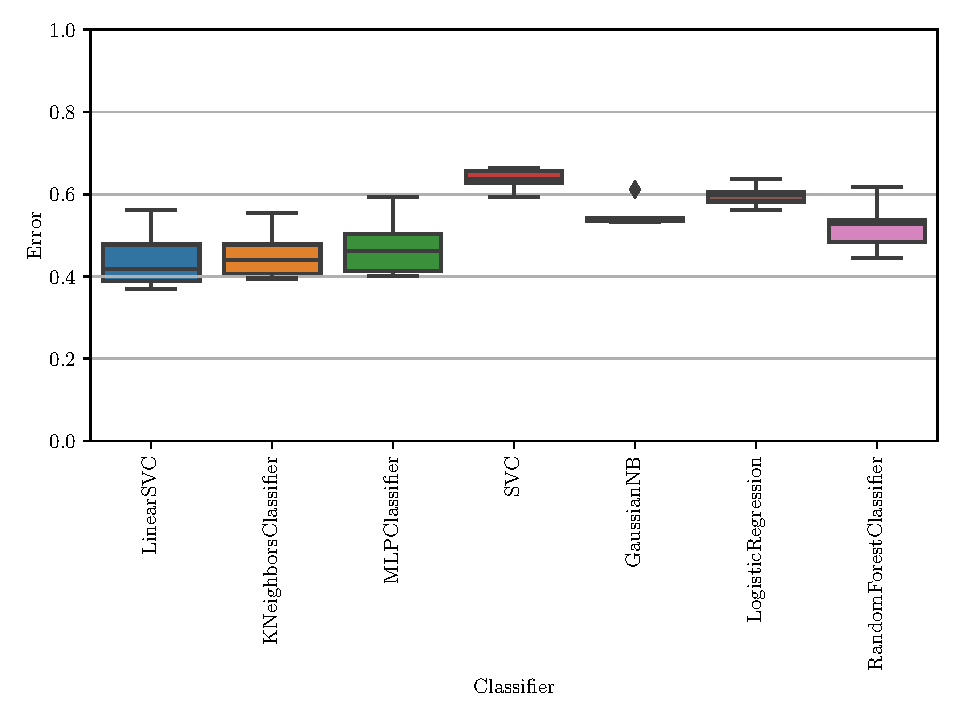
\includegraphics[width=\scale\textwidth]{../img/plot_explore_classifiers.pdf}
  \caption{Performance of classifiers without GridSearchCV optimization.}
  \label{fig:explore_classifiers}
\end{figure} 

The LinearSVC classifier performed best compared to other classifiers and it is a fast running algorithm even with data that has many features. We decided to look further into LinearSVC because it performed so well. We also wanted to conduct more testing with KNeighborsClassifier and Neural Networks. 

We created three models for LinearSVC, the first was a boilerplate LinearSVC with no argument modifications, the second model used the class weights parameter set to 'balanced'. The 'balanced' mode uses the values of y to automatically adjust weights inversely proportional to class frequencies in the input data as $n\_samples / (n\_classes * np.bincount(y))$. 

For the third test we created a dictionary of weights for each class using the Cosine decay function. The weights for each category ranged from 0.1 to 1.0 where the most frequent classes had smaller weights. The Cosine decay function is defined as:

\begin{equation}
    w_i = \frac{1}{2} \left(1 + \cos \left(\frac{\pi t}{T}\right)\right)
\label{eq:cosine_decay}
\end{equation}

where $w_i$ is the weight for the $i^{th}$ class, $t$ is the current iteration, and $T$ is the total number of iterations. The Cosine decay function is a common function used for weights in machine learning algorithms. The calculated cosine weights are shown in Figure \ref{tab:cosine_decay_weights}.

\begin{table}[!ht]
\centering
\caption{Cosine decay weights for each category.}
\begin{tabular}{lr}
\toprule
{} &  Weight \\
\midrule
Shopping Online       &   1.000 \\
Investments           &   0.996 \\
Drugstore             &   0.983 \\
Atm                   &   0.963 \\
Financial Services    &   0.934 \\
Children              &   0.899 \\
Freetime              &   0.857 \\
Bills And Household   &   0.810 \\
Culture               &   0.757 \\
Sport                 &   0.701 \\
Electronics           &   0.642 \\
Digital Services      &   0.581 \\
Pets                  &   0.519 \\
Fashion               &   0.458 \\
Consumer Goods        &   0.399 \\
Beauty                &   0.343 \\
Professional Services &   0.290 \\
House And Garden      &   0.243 \\
Travel                &   0.201 \\
Health                &   0.166 \\
Groceries             &   0.137 \\
Car                   &   0.117 \\
Food And Drink        &   0.104 \\
\bottomrule
\end{tabular}

\label{tab:cosine_decay_weights}
\end{table}

The results for the LinearSVC classifier experiments are shown in Table \ref{tab:lsvc_errors} where the LinearSVC with the Cosine decay weights performed just slightly better than the unmodified LinearSVC.

\begin{table}[!ht]
\centering
\caption{Error for three differing LinearSVC models.}
\begin{tabular}{lr}
\toprule
               Model &  Error \\
\midrule
Cosine Decay Weights &  0.392 \\
         Boilerplate &  0.407 \\
    Balanced Weights &  0.441 \\
\bottomrule
\end{tabular}

\label{tab:lsvc_errors}
\end{table}

Using K-Neighbors Classifier (KNN) and a Neural Network from TensorFlow we conducted additional experiments. For the KNN we found that using 8 neighbors and the cosine distance metric provided the lowest error. 

For the Neural Network we used a dense hidden-layer with 1000 neurons with Sigmoid activation and 23 output neurons with Softmax activation. For the NN optimizer we used Adamax with Cosine decay with an initial learning rate of 0.1, alpha value of 0.1 and 915 decay steps ($X\_data\_size // batch\_size * num_epochs$). The results are shown in Table \ref{tab:best_errors}. We can see that the K-Nearest Neighbors classifier and the Neural Network classifier performed slightly worse compared to LinearSVC.

The LinearSVC outperformed the other classifiers and we decided to experiment with it further. We attempted to boost performance of the LinearSVC classifier using multiple cross validation grid searches with the bagging. Bagging (bootstrap aggregating) is a type of ensemble learning, where multiple models are trained on different subsets of the training data and their predictions are combined to make the final prediction. In Scikit-Learn we used the BaggingClassifier to implement bagging. An example of our setup and parameters are shown in the code snippet. 

\begin{lstlisting}[language=Python]
base_classifier = LinearSVC()
bagging_classifier = BaggingClassifier(
    base_estimator = base_classifier,
    n_estimators = 20, 
    random_state = args.seed)
params = {
    'base_estimator__random_state': [args.seed],
    'base_estimator__max_iter': [10000],
    'base_estimator__intercept_scaling': 
        np.linspace(0.1, 1, 20),
    'base_estimator__loss': ['hinge', 'squared_hinge'],
    'base_estimator__penalty': ['l1', 'l2'],
    'base_estimator__class_weight': [None, weights],
    'base_estimator__C': np.linspace(0.1, 1000, 50),
    'base_estimator__multi_class': ['ovr', 
        'crammer_singer']
    }
\end{lstlisting}

Performance was not improved from what we had already seen. Using bagging may not be the best approach at this stage because there are some categories that have very few samples so bagging may be unable to create a good model. We will revisit bagging in future chapters when we have more data at our disposal. We also didn't use the balanced class weights parameter because we had already seen that it was the worst performing class weight parameter in previous tests. The BaggingClassifier and GridSearchCV combination didn't improve the performance of the LinearSVC classifier beyond what we had already achieved.

\begin{table}[!ht]
\centering
\caption{Testing errors for best performing classifiers.}
\begin{tabular}{lr}
\toprule
         Model &  Error \\
\midrule
     LinearSVC &  0.392 \\
Neural Network &  0.446 \\
           KNN &  0.451 \\
\bottomrule
\end{tabular}

\label{tab:best_errors}
\end{table}

The precision-recall curve for the best performing classifier (LinearSVC) is shown in Figure \ref{fig:pr_curve} and the confusion matrix is shown in Figure \ref{fig:confusion_matrix} for the best performing LinearSVC classifier.The precision-recall curve gives us an idea at how well our classifier can correctly categorize the data. It also gives us a visualization of how unbalanced our categories are. We can see this imbalance clearly in Figure \ref{fig:pr_curve} where we have straight lines and large steps for some categories. This is a result of having a small number of data in a class. However, we can also see that for some classes the precision is relatively high even though we have few data points. Here we are namely concerned with the 'Culture' and 'Beauty' categories which have 10 and 31 data points respectively. It may be that the keywords in the 'Culture' and 'Beauty' categories are drastically different from the other categories so the performance is better. 

\begin{figure}[ht]
  \centering
  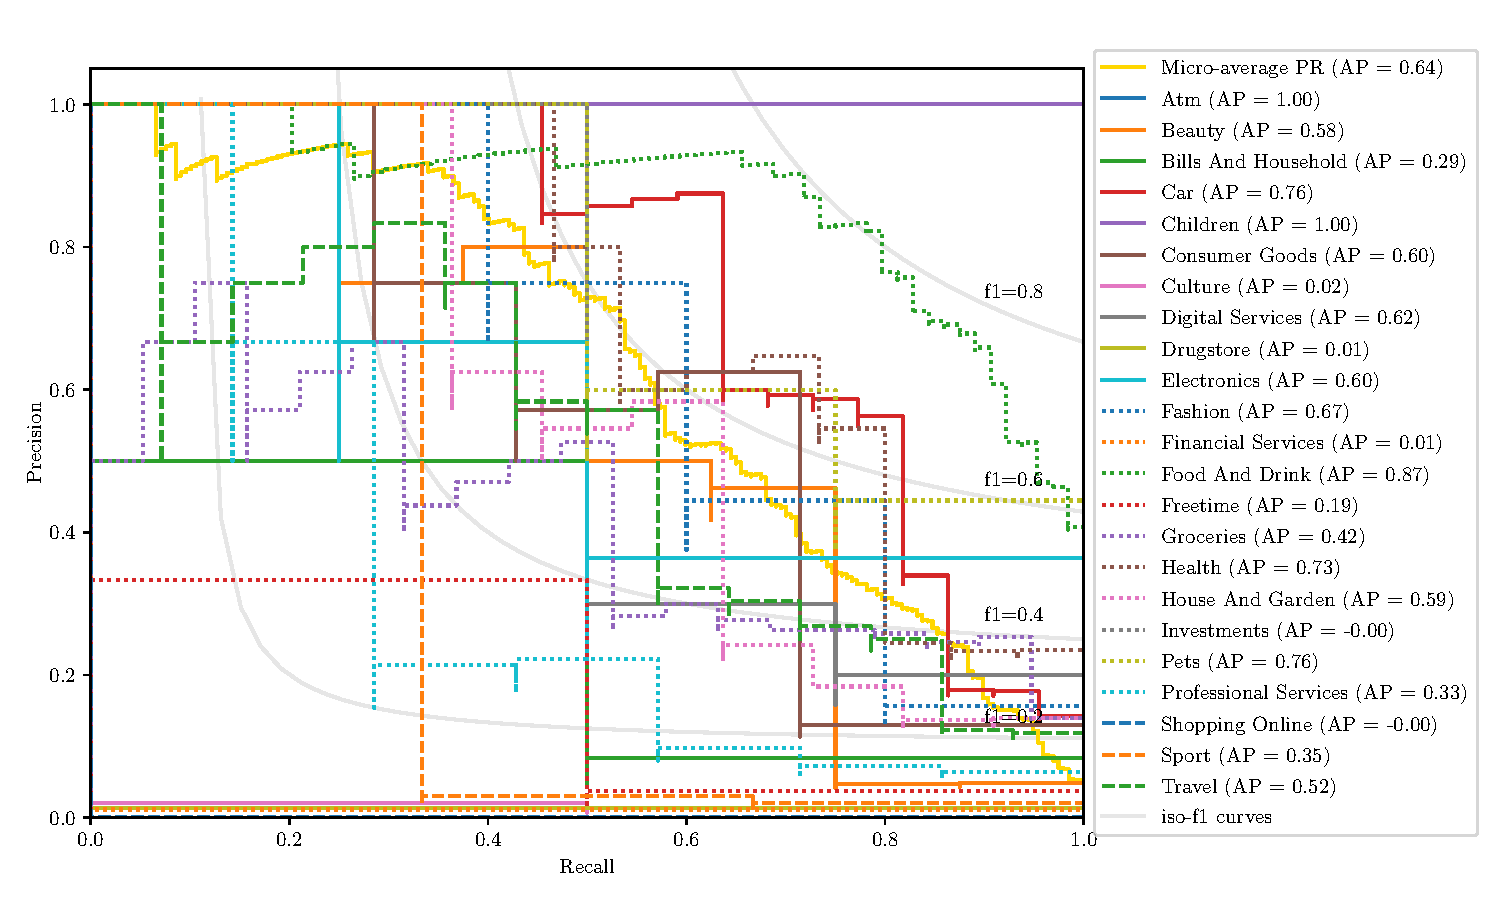
\includegraphics[width=\scale\textwidth]{../img/plot_pr_curve.pdf}
  \caption{Precision-recall curve for the best performing LinearSVC classifier.}
  \label{fig:pr_curve}
\end{figure}


The confusion matrix shown in Figure \ref{fig:confusion_matrix} may be a better metric for visualizing this data. In addition, the classification report for the LinearSVC classifier is shown in Appendix Table \ref{tab:classification_report_LinearSVC} with F1, accuracy, precision, recall, and support scores.

\begin{figure}[ht]
  \centering
  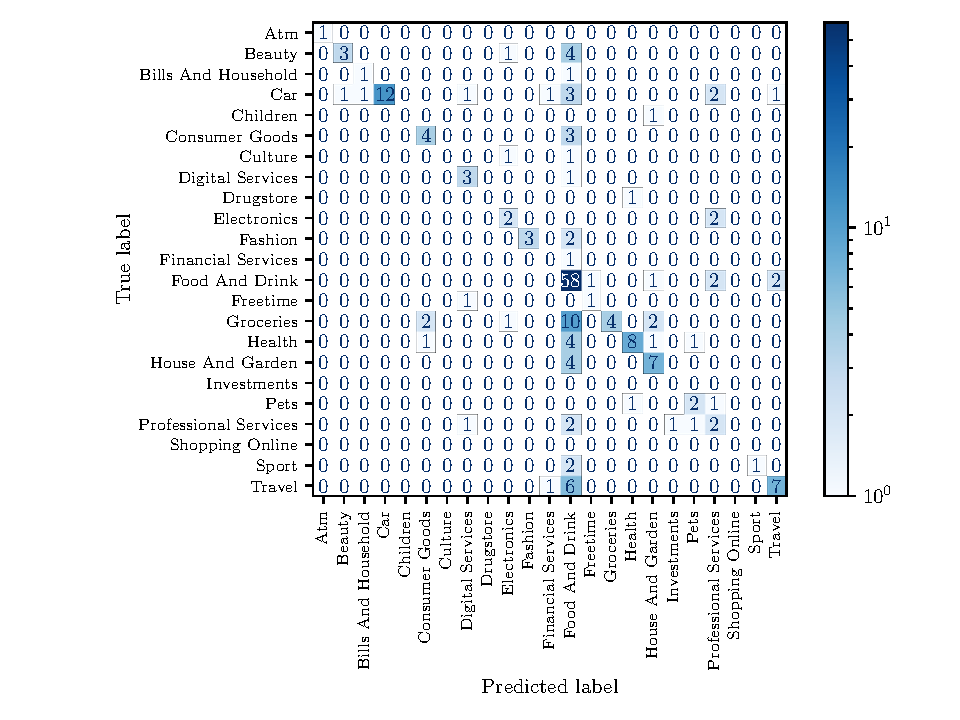
\includegraphics[width=\scale\textwidth]{../img/plot_cm_LinearSVC.pdf}
  \caption{Confusion matrix for the best performing LinearSVC classifier.}
  \label{fig:confusion_matrix}
\end{figure}


\section{Original and Additional Data}

In this section we will take what we have learned from the experiments in the previous sections and apply that knowledge to the original data set augmented with the additional data that we collected. This will provide us with a better understanding of how the data is interacting with the active learning sampling strategies and the PWC classifier. We will also experiment with removing some data from the set if the scraped text is less than a certain length and see if we can find a text length hyper parameter that maximizes performance.

\subsection{Active Learning with Additional Data}

In this first experiment we tested all the active learning methods with the new TF-IDF vectorizer that was fitted to the original data and the additional data. We then used this vectorizer to transform the original and additional data then saved the data into separate csv files. Next, using the active learning code from \cite{kottke2021toward} we constructed the train and test sets to split the original data the same way as in the previous active learning experiments.  

We then combined the original and additional data and used the different active learning methods and PWC with the Cosine kernel to train the classifiers. We used the same seeds as before and ran 10 test runs for each method and then averaged the test error of all the runs resulting in a single curve for each sampling strategy. We only used the first 612 data points to align with our previous experiments. As a result, the test error doesn't converge in this plot because we are only using a subset of the data. The results are shown in Figure \ref{fig:active_learning_new_data_new_vect}

\begin{figure}[ht]
  \centering
  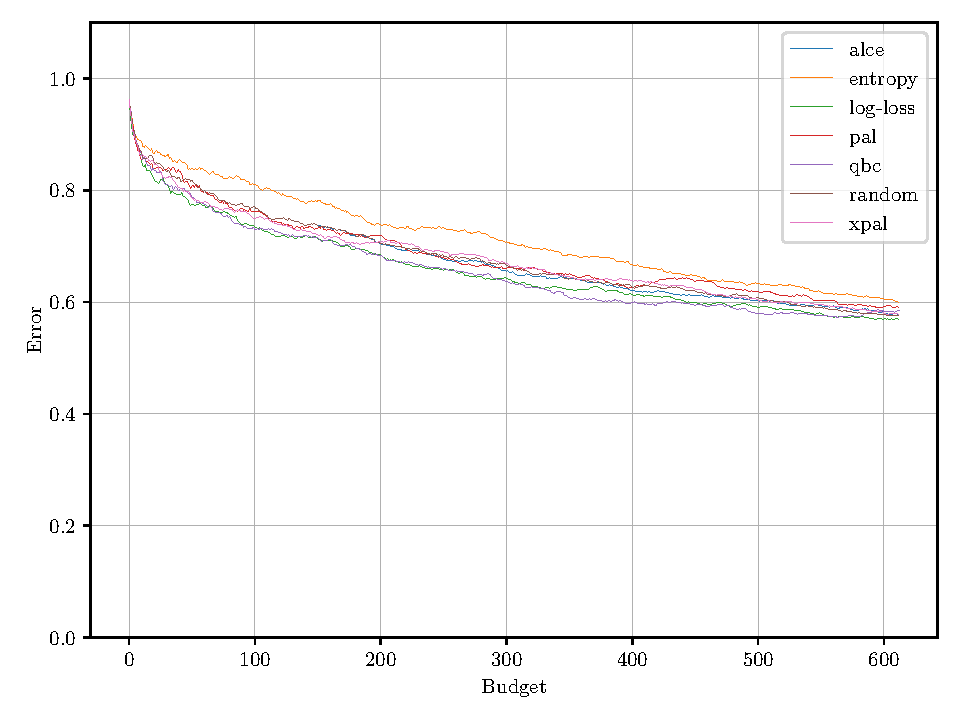
\includegraphics[width=\scale\textwidth]{../img/plot_all_data_new_vectorizer_test_results.pdf}
  \caption{Active learning results with using all data, 'xpal-original' curve from previous experiments is added for reference.}
  \label{fig:active_learning_new_data_new_vect}
\end{figure}

Its clear that active learning sampling strategies found it more difficult with this additional data compared to our previous runs. We can clearly see that the xpal-original outperformed all other sampling strategies.

When making more data available to the classifier we assumed that the test error would decrease. However, it may be the case that the additional data is not as useful as we thought.

\subsection{LinearSVC with Additional Data}

We have some data that may not have enough text to classify correctly and others that have more than 1000 characters of text that may be noisy. In addition we now have the luxury of having more than the minimum of 2 data points in some categories. We decided to explore if filtering the data based on text length could improve the performance of the classifier and use LinearSVC with weights as it has performed well with this data previously and it is relatively fast to train.

We imported the data and either selected a minimum number of characters or we altered the maximum number of characters allowed and created a new dataset. For each run we selected the data based on this criteria and then built the TF-IDF array. For the minimum string size tests we incremented the string size by 5 characters. While for the max string size tests we incremented the string size by -10. We again used a train test split of 25\% which has been our standard for testing throughout our experiments. We found that around the 200 character mark we would filter out too much data and would not have a minimum representation (2 data points) for all the categories. 

The filtered data set has 554 data points and 'Drugstore' is the only category that had 2 data points. The results for this experiment are shown in Figure \ref{fig:grid_search_text_length}. It is clear that the performance is better when we have a minimum text length requirement of 155 characters and no maximum text length requirement. 

\begin{figure}[ht]
    \centering
    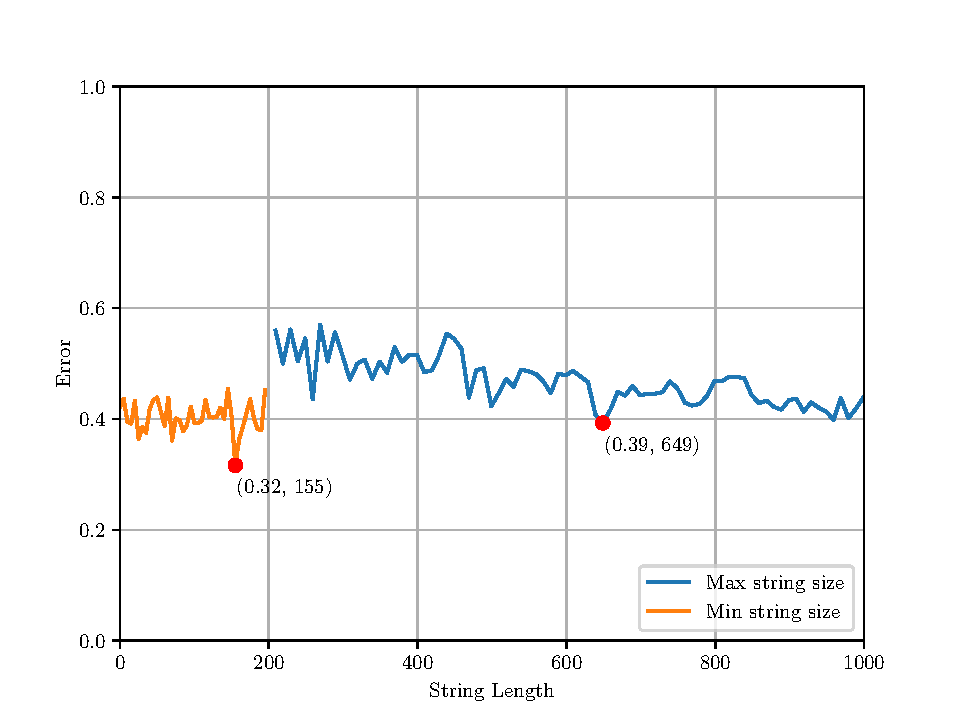
\includegraphics[width=\scale\textwidth]{../img/plot_data_length_grid_search.pdf}
    \caption{Performance results for best LinearSVC with varying text length parameters using all available data.}
    \label{fig:grid_search_text_length}
  \end{figure}

We we're able to reduce the test error by approximately 7.6\% using the LinearSVC and the minimum text length requirement. We also tested with a minimum text length and a maximum text length constraint implemented together but this combination did not improve the performance further.

\subsection{Active Learning Revisited}

With the new filtered data set we also wanted to see how the PWC classifier with active learning would perform. We used the same text length constraints as before and ran the PWC classifier with the Cosine kernel. The results for these experiments are shown in Figure...



